\section{Bug Detector}\label{sec:checker}

\begin{table}
  \centering
  \caption{Type-related specification bugs fixed by pull requests for the recent
  three years from 2018 to 2021}
  \label{table:pr-bugs}
  \vspace*{-1em}
  \[
\renewcommand{\arraystretch}{1.2}
    \begin{array}{c|l|r|r}
      \multicolumn{1}{c|}{\textbf{Category}} &
      \multicolumn{1}{c|}{\textbf{Bug Kind}} &
      \multicolumn{1}{c|}{\textbf{\# Pull Requests}} &
      \multicolumn{1}{c}{\textbf{\# Bug Fixes}}\\
      \hline \hline

      \multirow{2}{*}{\stextsf{\footnotesize Reference}}
      & \stextsf{\footnotesize UnknownVar} & 5 & 12\\\cline{2-4}
      & \stextsf{\footnotesize DuplicatedVar} & 2 & 12\\\hline

      \multirow{1}{*}{\stextsf{\footnotesize Arity}}
      & \stextsf{\footnotesize MissingParam} & 2 & 4\\\hline

      \multirow{1}{*}{\stextsf{\footnotesize Assertion}}
      & \stextsf{\footnotesize Assertion} & 4 & 5\\\hline

      \multirow{2}{*}{\stextsf{\footnotesize Operand}}
      & \stextsf{\footnotesize NoNumber} & 1 & 2\\\cline{2-4}
      & \stextsf{\footnotesize Abrupt} & 5 & 6\\\hline \hline

      \multicolumn{2}{c|}{\textbf{Total}} & 19 & 41\\

    \end{array}
  \]
  \vspace*{-1.5em}
\end{table}

We develop a \textit{bug detector} to statically detect type-related
specification bugs in ECMAScript using an augmented abstract transfer function
$\detector$ with additional checkers.  Before implementing checkers, we manually
investigated pull requests for the recent three years from 2018 to 2021 to identify
important bugs to detect.  As summarized in Table~\ref{table:pr-bugs},
we found 19 pull requests that fixed 41 type-related specification bugs,
and classified the bugs into four categories with six kinds.
To detect them automatically, we implement four checkers:
a \textit{reference checker}, an \textit{arity checker},
an \textit{assertion checker}, and an \textit{operand checker}.

\subsection{Reference Checker}

ECMAScript abstract algorithms dynamically introduce variables in any contexts.
A \textit{reference bug} occurs when trying to access variables not yet defined (\stextsf{UnknownVar})
or to redefine variables already defined (\stextsf{DuplicatedVar}).
According to our manual investigation of the pull requests,
the reference bug is the most prevalent type-related specification bugs;
five pull requests fixed 12 unknown variable bugs and two pull requests fixed
12 duplicated variable declaration bugs.  We implement a reference checker by adding
additional checks to the abstract semantics of variable lookups and variable
declarations as follows:
\begin{figure}[H]
  \centering
  \vspace*{-0.5em}
  \resizebox{\columnwidth}{!}{$
    \begin{array}{@{}l@{~}c@{~}l@{}}
      \aseme{\x}(\aenv) &=& \left\{
        \begin{array}{ll}
          \text{unknown variable} \; $\x$
          & \text{if} \; \asemr{\x}(\aenv) = \{ \tabsent \}\\
          \cdots
          & \text{otherwise}\\
        \end{array}
      \right.\\

      \asemi{\kwlet \; \x = \expr}(\lab, \tys)(\aelem) &=& \left\{
        \begin{array}{ll}
          \text{already defined variable} \; $\x$
          & \text{if} \; \aty = \{ \true \}\\
          \cdots
          & \text{otherwise}\\
        \end{array}
      \right.\\ &&
      \text{where} \; \aty = \aseme{\x \kwexists}(\aelem(\lab, \tys))\\
    \end{array}
  $}
  \vspace*{-0.5em}
\end{figure} \noindent
If the abstract semantics of a variable lookup for $\x$ is a singleton $\{ \tabsent \}$,
$\x$ is always an unknown variable.  For example, consider the syntax-directed algorithm
in Figure~\ref{fig:example}(a).
Since the \textbf{GetReferencedName} algorithm is removed, the variable
\code{GetReferencedName} does not exist in abstract environments and its lookup
returns $\{ \tabsent \}$. Thus, the reference checker reports the unknown variable
bug for \code{GetReferencedName}.  For duplicated variable declarations,
the reference checker utilizes the abstract semantics of the existence check
$\aseme{\x \kwexists}$ to see whether the variable $\x$ of each variable declaration is
already defined.


\begin{figure*}
  \centering
  \begin{subfigure}[b]{0.24\textwidth}
    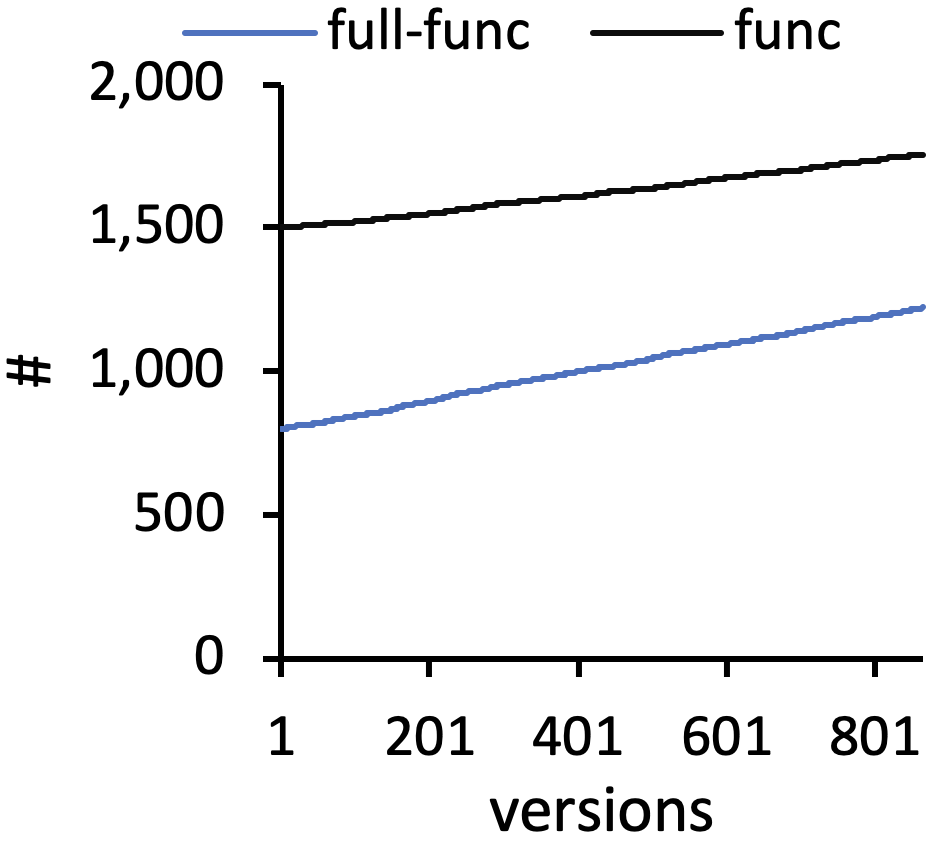
\includegraphics[width=\textwidth]{img/func}
    \caption{The number of functions}
  \end{subfigure}
  \begin{subfigure}[b]{0.24\textwidth}
    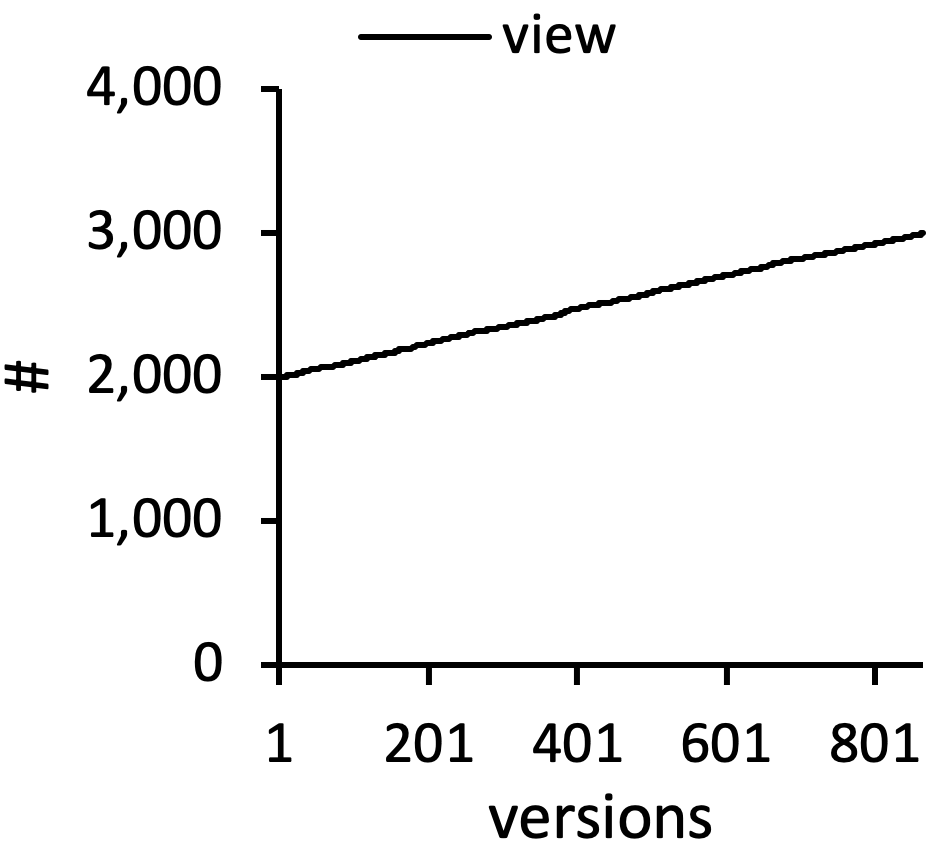
\includegraphics[width=\textwidth]{img/view}
    \caption{The number of views}
  \end{subfigure}
  \begin{subfigure}[b]{0.24\textwidth}
    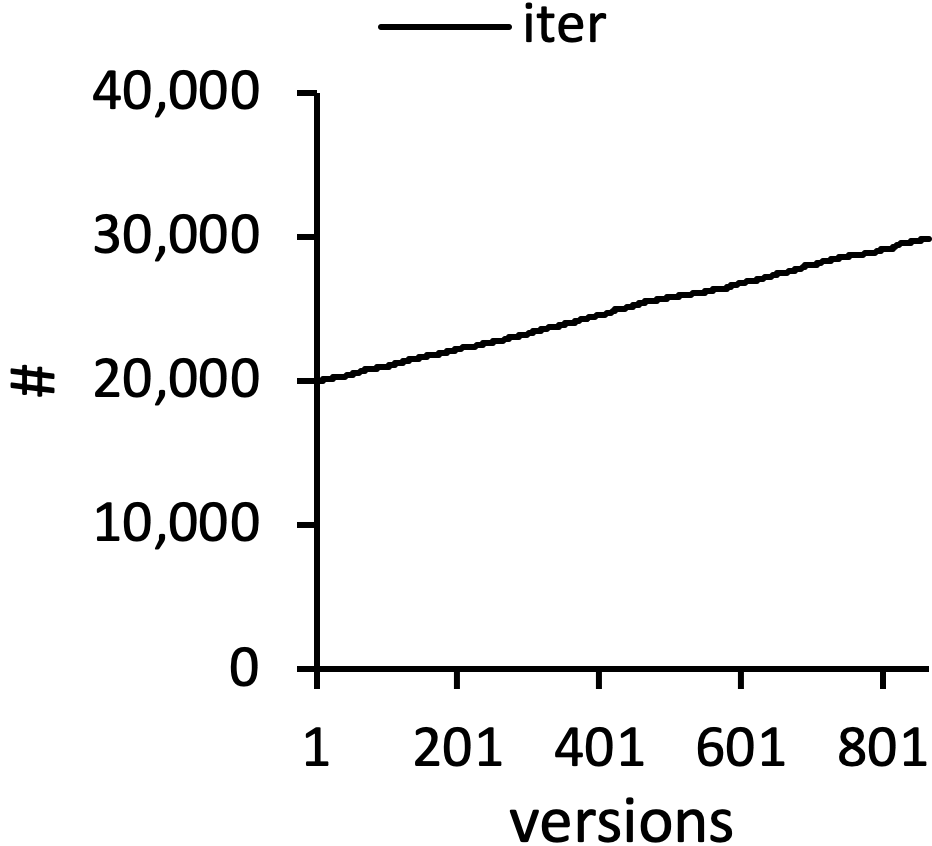
\includegraphics[width=\textwidth]{img/iter}
    \caption{The number of iterations}
  \end{subfigure}
  \begin{subfigure}[b]{0.24\textwidth}
    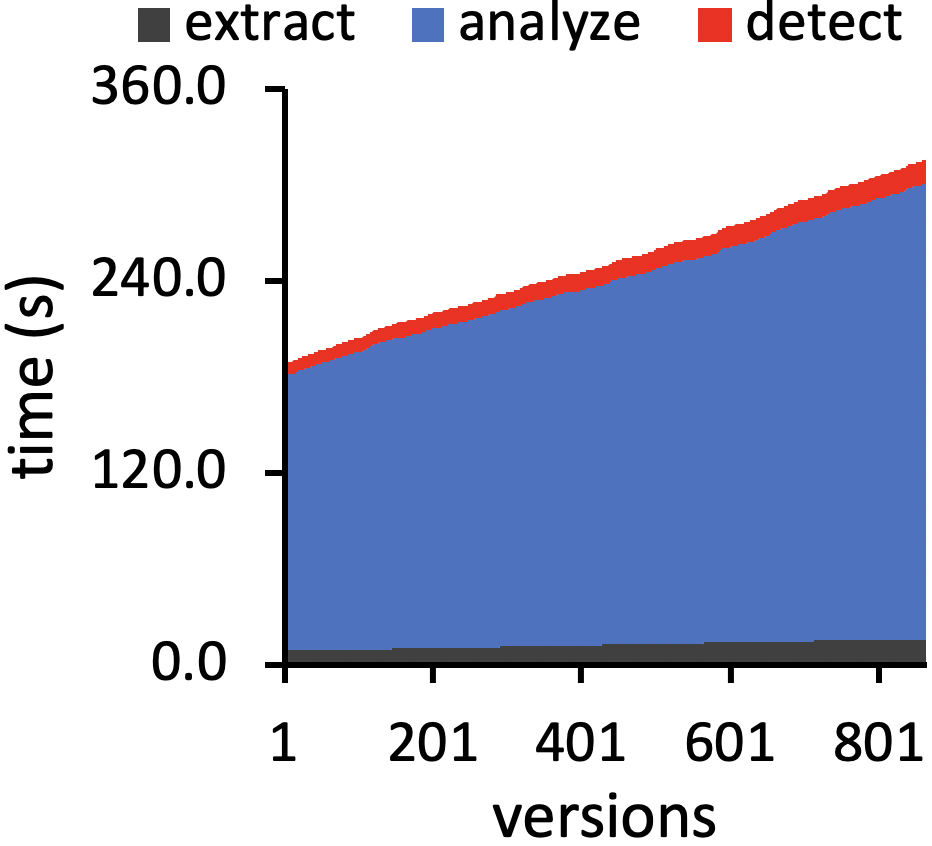
\includegraphics[width=\textwidth]{img/time}
    \caption{The analysis time}
  \end{subfigure}
  \caption{The statistics of the type analysis using $\tool$ for 864 versions of
  ECMAScript}
  \vspace*{-1em}
  \label{fig:stat}
\end{figure*}


\subsection{Arity Checker}

The arity of a function \mbox{\small
$\func = \kwfunc{\f}{\p_1, \cdots, \p_n, \kwsl \cdots, p_m \kwsr}{\lab}$}
is an interval $[n, m]$ where $n$ and $m-n$ denote the
numbers of normal and optional parameters, respectively.
In function invocations, an \textit{arity bug} occurs when
the number of arguments does not match with the function arity (\stextsf{MissingParam}).
In the last three years, two pull requests fixed four missing parameter bugs.
The arity checker detects them by adding an additional check to the abstract semantics of
the function call instruction:
\begin{figure}[H]
  \centering
  \vspace*{-0.5em}
  \resizebox{\columnwidth}{!}{$
    \begin{array}{@{}l@{}}
      \asemi{\x = \kwrl \expr \; \expr_1 \cdots \expr_k \kwrr}(\lab,
      \tys)(\aelem) =\\
      \qquad \left\{
        \begin{array}{ll}
          \text{missing parameters} \; \p_{k+1}, \cdots, \p_{n_\func} &
          \text{if} \; \exists \func \in \aty. \;\text{s.t.}\; k < n_\func\\

          \cdots &
          \text{otherwise}\\
        \end{array}
      \right.\\
      \qquad \text{where} \; \func = \kwfunc{\f}{\p_1, \cdots, \p_{n_\func},
      \kwsl \cdots, p_{m_\func} \kwsr}{\lab} \;\wedge\;\\
      \qquad \phantom{\text{where}} \; \aty = \aseme{\expr}(\aelem(\lab,
      \tys)).\\
    \end{array}
  $}
  \vspace*{-0.5em}
\end{figure} \noindent
For each function $\func$ in the abstract semantics of the function expression
$\expr$, the arity checker compares the number of arguments with the arity of
$\func$ to detect missing parameters.  For example, consider the
syntax-directed algorithm in Figure~\ref{fig:example}(b).  The algorithm invocation
on line 2 is compiled to the following function call instruction:
\[
  \fcode{x = (formals.IteratorBindingInitialization formals)}
\]
using a temporary variable $\x$.  Because it passes only a single argument
$\code{formals}$ even though the function arity is $[3, 3]$, the arity checker reports
missing parameter bugs for two additional parameters $\code{iteratorRecord}$ and
$\code{environment}$.


\subsection{Assertion Checker}
An \textit{assertion failure} (\stextsf{Assertion}) is a specification bug that
occurs when the condition of an assertion instruction is not true.
We found four pull requests that fixed five assertion failures.
The assertion checker detects them using an additional check in the
abstract semantics of the assertion instruction:
\begin{figure}[H]
  \centering
  \vspace*{-0.5em}
  \resizebox{0.95\columnwidth}{!}{$
    \begin{array}{@{}l@{~}l@{}}
      \asemi{\kwassert \; \expr}(\lab, \tys)(\aelem) = & \left\{
        \begin{array}{ll}
          \text{assertion failure} \; \expr &
          \text{if} \; \{ \true \} \norder \aty\\

          \cdots &
          \text{otherwise}\\
        \end{array}
      \right.\\ &
      \text{where} \; \aty = \aseme{\expr}(\aelem(\lab, \tys))\\
    \end{array}
  $}
  \vspace*{-0.5em}
\end{figure} \noindent
It checks whether the abstract semantics of the condition expression $\expr$ 
subsumes $\{ \true \}$.  For example, consider the syntax-directed
algorithm in Figure~\ref{fig:example}(c).  The parameter $\code{environment}$ of
this algorithm has an environment record or $\undefval$.
Since type sensitivity divides the abstract types of arguments to
upcasted single types, there are two different abstract environments whose
variable $\code{environment}$ points to $\{ \code{Environment} \}$ or $\{ \undefval \}$.
When $\code{environment}$ is $\{ \code{Environment} \}$, the
abstract semantics of the assertion condition $\code{environment = originalEnv}$ is $\{ \tbool \}$.
Even though we know that the type of $\code{originalEnv}$ is
also $\{ \code{Environment} \}$, because \code{Environment} is not a singleton type,
we cannot conclude that they are the exactly same environment.
Thus, the assertion checker does not report any bug for this case.
However, if $\code{environment}$ is $\{ \undefval \}$, the abstract semantics of the
condition $\code{environment = originalEnv}$ is $\{ \false \}$ because an
environment is never equal to $\undefval$.
Therefore, the assertion checker reports an assertion failure for
the condition $\code{environment = originalEnv}$.


\subsection{Operand Checker}

An \textit{ill-typed operand bug} occurs when
the type of an operand does not conform to its corresponding parameter type.
The operand checker detects such ill-typed operand bugs by additional
checks in the abstract semantics of operations:
\begin{figure}[H]
  \centering
  \vspace*{-0.5em}
  \resizebox{0.9\columnwidth}{!}{$
    \begin{array}{@{}l@{~}c@{~}l@{}}
      \aseme{\expr_0 \bop \expr_1}(\aenv) &=& \left\{
        \begin{array}{ll}
          \text{ill-typed operand} \; \expr_0
          & \text{if} \; \asemr{\expr_0}(\aenv) \norder \aty_0\\
          \text{ill-typed operand} \; \expr_1
          & \text{if} \; \asemr{\expr_1}(\aenv) \norder \aty_1\\
          \cdots
          & \text{otherwise}\\
        \end{array}
      \right.\\

      \aseme{\uop \; \expr}(\aenv) &=& \left\{
        \begin{array}{ll}
          \text{ill-typed operand} \; \expr\ \ \,
          & \text{if} \; \asemr{\expr}(\aenv) \norder \aty\\
          \cdots
          & \text{otherwise}\\
        \end{array}
      \right.\\
    \end{array}
  $}
  \vspace*{-0.5em}
\end{figure} \noindent
where $\aty_0$, $\aty_1$, and $\aty$ are expected abstract types of $\expr_0$,
$\expr_1$, and $\expr$, respectively.  The additional checks report
when a given operand does not conform to its expected type.  According to our
manual investigation, there existed two different kinds of ill-typed operand
bugs: two non-numeric operand bugs (\stextsf{NoNumber}) in one pull request, and
six unchecked abrupt completion bugs (\stextsf{Abrupt}) in five pull requests.

For an example of non-numeric operand bugs, consider the built-in
algorithm $\code{Math.round}$ in Figure~\ref{fig:example}(d).  The types of $\x$
and $\n$ are $\{ \tjs \}$ and $\{ \tnum \}$, respectively, because the
\textbf{ToNumber} algorithm always returns number values or abrupt completions,
and the prefix \textbf{?} removes the latter case.  The built-in algorithm
misuses $\x$ rather than $\n$ on lines 3 and 4, and because the expected
abstract type $\{ \tnum, \tbigint \}$ does not subsume $\{ \tjs \}$, the operand
checker reports non-numeric operand bugs.

An unchecked abrupt completion bug occurs when the actual value is necessary but
it is an abrupt completion.  ECMAScript has a special implicit conversion for
normal completions when their actual values stored in the $\code{Value}$ field
are necessary, such as conditions, values of field updates, and operands of
operators.  For example, if the variable $\x$ has a normal completion with
\code{42} as its actual value, $\code{x + 1}$ should be \code{43} because the
normal completion gets implicitly converted into its actual value \code{42}.  To
explicitly represent this conversion, we define a unary operator $\escaped$ as
follows:
\begin{figure}[H]
  \centering
  \vspace*{-0.5em}
  \resizebox{\columnwidth}{!}{$
    \escaped \val = \left\{
      \begin{array}{ll}
        \val &
        \text{if} \; \val \; \text{is not a completion}\\

        \val.\code{Value} &
        \text{if} \; \val \; \text{is normal}\\

        \text{unchecked abrupt completion} \; \val &
        \text{otherwise}\\
      \end{array}
    \right.
  $}
  \vspace*{-0.5em}
\end{figure} \noindent
and assume that the operator $\escaped$ is used when the actual value is necessary.
